%%%%%%%%%%%%%%%%%%%%%%%%%%%%%%%%%%%%%%%%%
% Beamer Presentation
% LaTeX Template
% Note:
% data cleaning should be added
% https://realpython.com/python-data-cleaning-numpy-pandas/
% 


\documentclass{beamer}
\mode<presentation> {
\usetheme{Warsaw}
}

\usepackage{multicol}
\usepackage[russian]{babel}
\usepackage{graphicx} 
\usepackage{hyperref}

\title[Introduction to Python]{Control Flow} 
\author{Sugarkhuu Radnaa} 
\institute[]
{
Py4Econ in Ulaanbaatar \\ 
\medskip
\textit{py4econ@gmail.com} 
}
\date{}  %15 January, 2022 \today

\begin{document}

\begin{frame}
\titlepage % Print the title page as the first slide
\end{frame}

\begin{frame}
    \frametitle{Week 5: Learning objectives}
    Get to know: 
    \begin{enumerate}
        \item \textbf{if, else and elif} conditions
        \item \textbf{for and while} loop
        \item Useful tips
    \end{enumerate}
\end{frame}

%------------------------------------------------
\section{Control Flow} 
%------------------------------------------------

\begin{frame}
    \frametitle{Contiditional statements}
    \begin{itemize}
        \item if statement:
        \item else:
        \item elif (else if) statement:  
        \item and, or, in, isinstance
    \end{itemize}
\end{frame}

\begin{frame}
    \frametitle{Loops (repeat an action)}
    \begin{itemize}
        \item For - used only when we already knew the number of iterations
        \item While - used only when the number of iteration are not exactly known
    \end{itemize}

    Ways to exit loop:
    \begin{itemize}
        \item break
        \item continue
    \end{itemize}
    
    Use 'pass' when operation within the loop is not implemented yet
\end{frame}

\begin{frame}
    \frametitle{USEFUL TIPS: One liner and Lambda}
        Helpful for writing concise codes
            \begin{center}
                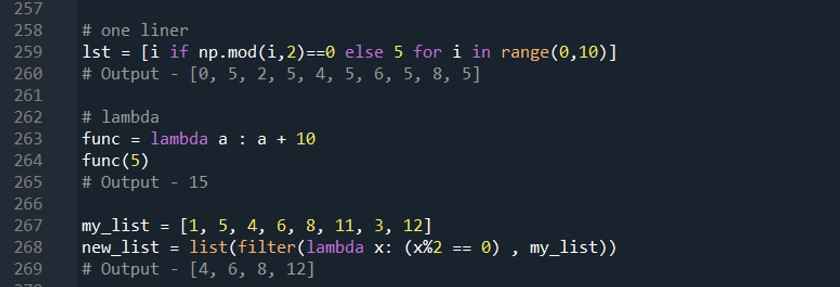
\includegraphics[scale=0.5]{figures/one_liner.jpg}
            \end{center}
    \end{frame}

%------------------------------------------------
\section{Homework} 
%------------------------------------------------

\begin{frame}
    \frametitle{Homework}
    \begin{enumerate}
        \item Task 1
        \item Task 2
        \item Task 3
        \item Task 4 
    \end{enumerate}

    \vskip 2mm
    \begin{itemize}
        \item Submit your result as a Github repository
        \item Deadline: 1 week %22 January, 2022
    \end{itemize}

\vfill
\textbf{Note:} Create a github repo from the start and populate it with your results step by step.
\end{frame}

\begin{frame}
    \frametitle{Task 1}
    Using 'data.xlsx' with 'if' and 'for' loop, do the following:
    \begin{enumerate}
        \item Create a '.csv' file with data of only women older than 25 years old
        \item Create a '.json' file with data of men under than 23 years old
    \end{enumerate}
\end{frame}

\begin{frame}
    \frametitle{Task 2}
    Using 'np.random.random\_integers' function, create a list of length 20 comprising of numbers between 50 and 60. 
    Then, do the following for the list:
    \begin{enumerate}
        \item Create a sublist consisting only of odd numbers (list, filter, lambda)
        \item Create a sublist consisting only of even numbers (list, filter, lambda)
        \item Create a list with all members multiplied by 10 (one-liner and map/lambda)
        \item Create a list where one is subtracted from odd numbers and even numbers stay as they are (one-liner)
        \item Print one of '$<$ 52','53-55','56-58' and '$>$59', respectively, for each number based on their value matches
        \item Print numbers one by one starting from the beginning until the first number above 58 appears (while)
        \item Print first 5 numbers using while loop (i += 1)
    \end{enumerate}
\end{frame}

\begin{frame}
    \frametitle{Task 3}
    Using 'data.xlsx', create two separate lists of first names and last names. Then, do the following:
    \begin{enumerate}
        \item Print out first name and last name next to each other using 'zip' command with loop 
        \item Print out first name and index of that next to each other using 'enumerate' command with loop 
    \end{enumerate}
\end{frame}

\begin{frame}
    \frametitle{Task 4: Optional}
    Do you find it manageable to solve the following problems?
    \begin{enumerate}
        \item https://pynative.com/python-if-else-and-for-loop-exercise-with-solutions/
        \item https://www.w3resource.com/python-exercises/python-conditional-statements-and-loop-exercises.php
    \end{enumerate}
\end{frame}





\begin{frame}
\Huge{\centerline{Thank you!}}
\end{frame}

%----------------------------------------------------------------------------------------

\end{document} 